% =============================================================================
%  重大活动交通态势洞察及辅助决策智能体集群 — 外部汇报版（八章精简）
% =============================================================================
%  编译方式：
%      xelatex report-brief.tex
%      latexmk -xelatex report-brief.tex
%
%  与内部版的对应关系：
%      • 内部完整版：report.tex                （八章正文 + 完整技术细节）
%      • 外部汇报版：report-brief.tex          （八章结构对齐 + 内容精简）
%
%  精简原则：
%      • 保留八章结构与编号，便于内外对照
%      • 业务场景截图集中在"七、结果展示"
%      • 技术选型与实现细节压缩为 1—2 段概述
% =============================================================================

\documentclass[a4paper,11pt]{article}

% --- 中文与字体 ---
\usepackage[UTF8,fontset=none]{ctex}
\setmainfont{texgyretermes-regular.otf}[
  BoldFont       = texgyretermes-bold.otf,
  ItalicFont     = texgyretermes-italic.otf,
  BoldItalicFont = texgyretermes-bolditalic.otf,
]
\setsansfont{texgyreheros-regular.otf}[
  BoldFont       = texgyreheros-bold.otf,
  ItalicFont     = texgyreheros-italic.otf,
  BoldItalicFont = texgyreheros-bolditalic.otf,
]
\setmonofont{texgyrecursor-regular.otf}
\setCJKmainfont{STSong}
\setCJKsansfont{STHeiti}
\setCJKmonofont{STFangsong}

% --- 页面布局 ---
\usepackage[a4paper,top=2.4cm,bottom=2.4cm,left=2.4cm,right=2.4cm]{geometry}
\usepackage{indentfirst}
\setlength{\parindent}{2em}
\linespread{1.3}

% --- 颜色与图形 ---
\usepackage{xcolor}
\usepackage{colortbl}
\usepackage{graphicx}
\graphicspath{{./}{./assets/}{./assets/重大活动交通态势洞察及辅助决策智能体集群/}}

\definecolor{ImportantColor}{RGB}{180,40,40}
\definecolor{WarnColor}{RGB}{200,140,0}
\definecolor{TableHead}{RGB}{230,235,240}

% --- 表格 ---
\usepackage{booktabs}
\usepackage{tabularx}
\usepackage{array}
\renewcommand{\arraystretch}{1.25}

% --- 列表 ---
\usepackage{enumitem}
\setlist[itemize]{leftmargin=1.5em,topsep=2pt,parsep=1pt,itemsep=1pt}
\setlist[enumerate]{leftmargin=1.8em,topsep=2pt,parsep=1pt,itemsep=1pt}

% --- 提示框 ---
\usepackage[most]{tcolorbox}
\newtcolorbox{admonition}[2]{
  enhanced, breakable,
  colback=#1!5!white, colframe=#1!75!black,
  fonttitle=\bfseries\sffamily, title={#2},
  boxrule=0.6pt, arc=2pt,
  left=8pt, right=8pt, top=4pt, bottom=4pt,
  before skip=8pt, after skip=8pt,
}
\newcommand{\importantbox}[1]{\begin{admonition}{ImportantColor}{重要提示}#1\end{admonition}}
\newcommand{\bordersbox}[1]{\begin{admonition}{WarnColor}{边界说明}#1\end{admonition}}

% --- 超链接与书签 ---
\usepackage[colorlinks=true,
            linkcolor=blue!60!black,
            urlcolor=blue!60!black,
            citecolor=blue!60!black,
            bookmarksnumbered=true,
            bookmarksopen=true]{hyperref}

% --- 标题格式 ---
\usepackage{titlesec}
\titleformat{\section}{\Large\bfseries\sffamily}{\thesection}{1em}{}
\titleformat{\subsection}{\large\bfseries\sffamily}{\thesubsection}{1em}{}
\titlespacing*{\section}    {0pt}{2.5ex plus 1ex minus .2ex}{1.2ex plus .2ex}
\titlespacing*{\subsection} {0pt}{1.8ex plus 1ex minus .2ex}{0.8ex plus .2ex}

% --- 页眉页脚 ---
\usepackage{fancyhdr}
\pagestyle{fancy}
\fancyhf{}
\fancyhead[L]{\small\sffamily 重大活动交通态势洞察及辅助决策智能体集群}
\fancyhead[R]{}
\fancyfoot[C]{\thepage}
\renewcommand{\headrulewidth}{0.4pt}

% --- 杂项命令 ---
\newcommand{\metarow}[2]{\textbf{#1} & #2 \\}
\newcommand{\code}[1]{\texttt{#1}}
\newcommand{\term}[1]{\textbf{#1}}

% =============================================================================
\begin{document}

% --- 封面 ---
\begin{titlepage}
\centering
\vspace*{2.5cm}

{\sffamily\bfseries\Huge 重大活动交通态势洞察\\[0.4em]及辅助决策智能体集群}\\[1.5em]

{\large\sffamily——以大型活动对重点场所（上海体育场）交通影响为例}\\[1.5em]

{\Large\bfseries\sffamily 项目建设说明报告}\\[1em]
{\small\sffamily\itshape 本报告为智能体“揭榜挂帅”题目下的产出}\\[2em]

{\small\sffamily
\textbf{\large 项目元信息}\\[4pt]
\rule{0.5\linewidth}{0.5pt}\\[8pt]
\begin{tabularx}{0.85\linewidth}{@{}lX@{}}
\metarow{系统名称}{TransportX Agent Workshop}
\metarow{研发团队}{同济大学 TransportX Lab}
\metarow{指导教师}{李健}
\metarow{数据支持}{EVDATA}
\metarow{案例对象}{2025 年 8 月上海体育场重大活动}
\metarow{编制日期}{2026 年 7 月 30 日}
\end{tabularx}
}

\vfill

{\footnotesize\sffamily 本报告依据仓库实现、数据资产说明与自动化测试结果编制。\\业务问数准确率与方案采纳率须经独立业务验收。\\道路交通管控措施由交通管理部门按职责依法审批。}

\vspace{1.5cm}
\end{titlepage}

% =============================================================================
%  一、总体概述
% =============================================================================
\section{总体概述}

\subsection{建设目标与定位}

本项目服务重大活动交通态势研判和保障决策。业务人员用自然语言提出问题，工作台查询授权范围内的数据，完成对比、制图和报告整理；每次任务保存数据来源、执行步骤和结果文件，复核时可以沿原路径回查。系统用于分析辅助，指挥和审批仍由交通管理部门负责。

项目建设围绕三个目标展开：\term{看得见}——把活动周边多源数据在地图和看板中直观呈现，让态势变化可被快速捕捉；\term{问得动}——以自然语言为入口，把业务问题转化为受控查询，避免人工拼接 SQL；\term{查得回}——把每次问数的过程、引用、产物沿原路径保存，便于审计与复核。

\subsection{场景描述与能力边界}

当前版本面向演唱会、体育赛事、大型集会等短周期、跨方式交通保障任务，覆盖五类业务能力：

\begin{itemize}
  \item \term{交通问数：}围绕业务口径理解自然语言问题，输出可核对的查询结果。
  \item \term{空间分析：}依托地图完成缓冲区、覆盖度、热点叠加与图层发布。
  \item \term{辅助研判：}联合问数与知识检索，按阶段生成可引用的方案建议。
  \item \term{知识检索与引用：}检索法规、预案、案例与项目资料，给出原文定位。
  \item \term{成果交付：}在同一会话内汇总报告、地图、引用与执行步骤。
\end{itemize}

\subsection{核心成果亮点概述}

系统围绕交通保障业务，重点在以下五个方面构建能力：

\begin{itemize}
  \item \term{一站分析。}在工作台内完成"提问—查询—地图—报告"完整链路，无需切换工具。
  \item \term{多源协同。}统一理解公交、轨交、道路、网约车、气象等多源数据。
  \item \term{态势直观。}围绕活动周边要素分层呈现，便于快速核对分布与变化。
  \item \term{可引用研判。}给出方案时同时给出依据，原文可定位可复核。
  \item \term{全程留痕。}保留完整的分析过程、步骤与产物版本，便于追溯与回看。
\end{itemize}

% =============================================================================
%  二、总体技术架构
% =============================================================================
\section{总体技术架构}

\subsection{总体架构设计}

系统围绕"提出问题、查看态势、研判方案"组织能力，由统一工作台、能力 harness、受控能力和支撑资源四个部分组成。业务人员通过一个入口完成提问、任务跟踪、地图查看和成果确认；Agent 根据任务调用数据、知识和分析工具；分析结果返回工作台后可继续追问或确认方案。

\begin{figure}[ht]
  \centering
  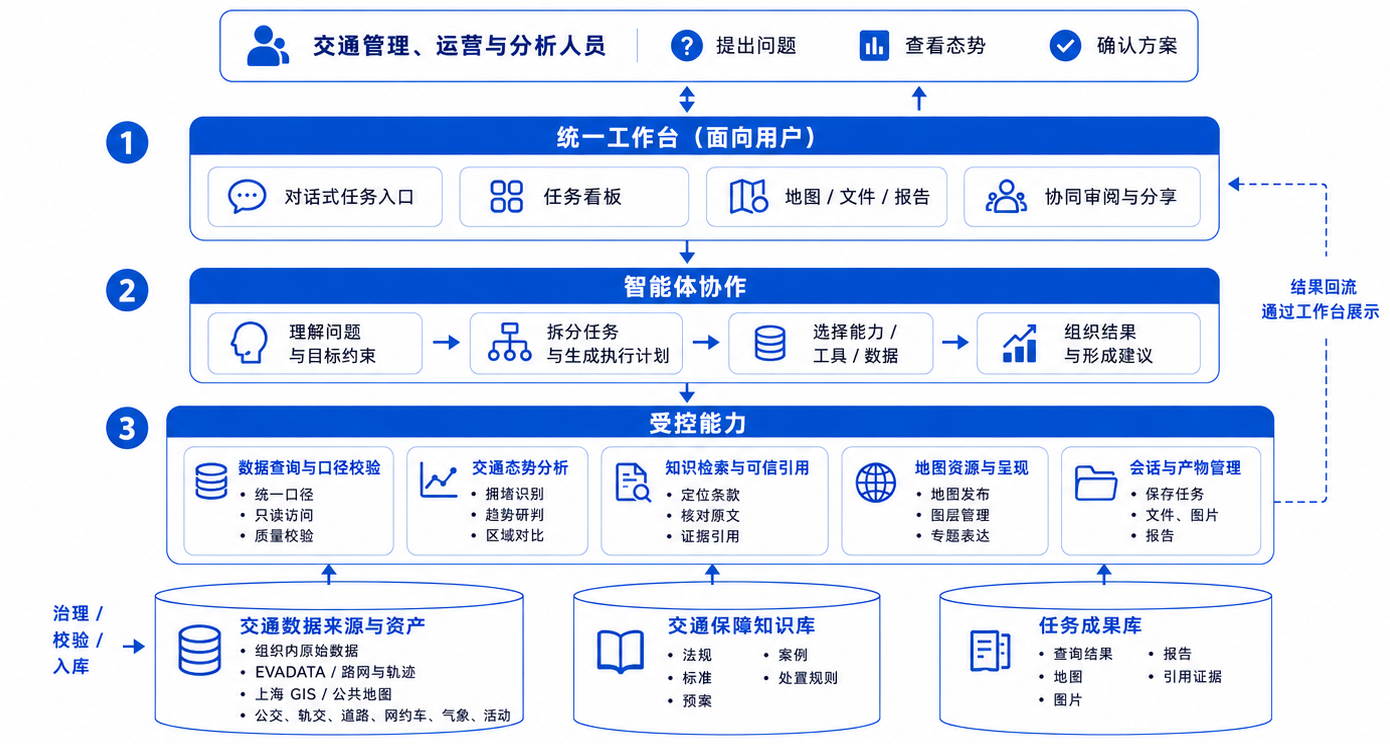
\includegraphics[width=0.92\linewidth]{00-overall-architecture.png}
  \caption{总体架构（工作台 / 能力 harness / 受控能力 / 支撑资源）}
  \label{fig:architecture}
\end{figure}

\subsection{分层模块说明}

工作台承接业务人员的所有交互；能力 harness 围绕当前任务调用问题理解、任务规划、数据查询、知识检索等能力；受控能力层把操作转化为明确的查询、分析和发布动作，数据库只读、地图命令与文件路径受规则约束；支撑资源由交通数据、交通保障知识库和任务成果组成。

\subsection{核心技术选型}

智能体运行时采用项目自研的轻量级 Agent Loop，专注于工具调用与任务步骤管理。Loop 围绕单会话内的多轮驱动设计，结构简洁、按需装配，便于在受控环境下稳定运行。服务端与前端基于 TypeScript 生态构建，前端采用现代 React 栈；地图组件基于 MapLibre GL 与 GeoScene，通过结构化命令驱动图层更新；数据存储采用 SQLite 分域库配合 Python 治理脚本，便于本地部署与版本迭代。

% =============================================================================
%  三、数据接入与治理
% =============================================================================
\section{数据接入与治理}

\subsection{基础数据}

组织方提供的核心业务数据包括网约车订单（含场馆关联的到场和离场订单）、公交客流、轨交客流、道路状态事件和气象观测，整体覆盖约 21—22 天的活动窗口，所有业务时间按 Asia/Shanghai 解释。

\begin{table}[ht]
  \centering
  \small
  \begin{tabularx}{0.94\linewidth}{@{}lXl@{}}
    \toprule
    \rowcolor{TableHead}
    \sffamily\bfseries 数据源 & \sffamily\bfseries 主要内容 & \sffamily\bfseries 主要用途 \\
    \midrule
    网约车订单   & 场馆关联的到场/离场订单、起讫点与时间戳 & 散场热点、运力匹配 \\
    公交客流     & 线路与站点上下客量                       & 公交分担、线路影响 \\
    轨交客流     & 站点进出站量、换乘量                     & 轨交保障、限流评估 \\
    道路状态事件 & 拥堵、施工、管制事件                      & 路网研判、绕行建议 \\
    气象观测     & 降水、风速、能见度                        & 风险评估、方案提示 \\
    \bottomrule
  \end{tabularx}
  \caption{核心业务数据一览}
  \label{tab:core-data}
\end{table}

\subsection{外部接入与项目补充数据}

系统接入 EVDATA 获取实时路况；项目自行完成上海 GIS 与公开地图的采集和标准化，统一轨交、公交与道路的坐标和站序；时间维度由业务时间戳派生并对齐到分钟、15 分钟、小时和日；交通保障知识库收录法规、预案、案例与项目资料。

外部接入重点是实时路况与影响交通的天气变化；项目补充数据用于弥补公开数据的覆盖差异与坐标差异。GIS 数据统一到 WGS84，地图瓦片按 MVT/PMTiles 规范组织；时间维度以业务时间戳为基准派生，避免因系统时区导致的口径偏移。

\subsection{数据处理方式}

数据处理围绕统一时间、统一坐标、订单去重与质量断言展开。不同坐标系的输入统一转换为 WGS84；订单按原始订单号 SHA-256 合并为唯一订单；事实与集市从标准层派生，问数优先查询集市；默认输出聚合数据，敏感字段受规则约束。

\begin{itemize}
  \item \term{坐标统一。}所有输入先转换到 WGS84，再写入对应分域库。
  \item \term{订单去重。}原始订单号 SHA-256 假名化后作为唯一键，跨源合并。
  \item \term{派生分层。}按"原始层→标准层→事实→集市"逐层派生，问数优先查集市。
  \item \term{质量断言。}覆盖率、缺失率、口径偏差作为错误级规则，触发即阻断发布。
  \item \term{最小化输出。}默认输出聚合结果，敏感字段按规则脱敏。
\end{itemize}

% =============================================================================
%  四、核心功能设计
% =============================================================================
\section{核心功能设计}

本系统围绕一个 LLM Agent 构建能力 harness，Agent 在同一会话内按需调用智能问数、辅助决策、任务控制、数据治理与查询、知识检索与引用、地理可视化和报告与产物管理等能力。能力由项目级 Skill、Extension 工具和共享契约约束，工作台按会话隔离任务目录、状态和地图资源。

\subsection{智能问数能力}

智能问数能力包含语义解释、资产发现、受控查询、结果校验和结果表达。Agent 识别问题中的交通方式、实体、时间范围、空间范围和指标单位；订单与事件、站点与线路、活动日与演出时段等口径存在歧义时发起结构化询问。查询使用只读语句，校验对象名与返回行数，结果附带原始 SQL 与图表脚本，可在会话目录复核。

\subsection{辅助决策能力}

辅助决策能力基于问数结果与知识检索结果联合推理。复杂任务拆分为 2—8 个可检查步骤，分别对应演前、演出中与散场阶段；每步产出可核对的证据，方案按态势摘要、证据与判断、建议措施、执行条件、风险与待确认事项组织。道路管制、轨交限流、停运、警力部署等措施由相应责任部门确认。

\subsection{配套能力}

任务控制、数据治理与查询、知识检索与引用、地理可视化和报告与产物管理等配套能力由 Agent 按任务需要调用，确保复杂分析任务可以被分解、跟踪、归档与复用。

\subsection{可解释性与可追溯设计}

可解释性与可追溯围绕六个维度展开：过程可见、状态可恢复、数据可追溯、引用可核查、产物可复查、错误可诊断。研判结论附带原文引用，可从结论回溯到证据、引用条目和法规预案原文。

% =============================================================================
%  五、系统交互与成果呈现设计
% =============================================================================
\section{系统交互与成果呈现设计}

\subsection{对话交互系统设计}

工作台以交通任务为入口，提供"新建交通任务"主操作，并将交通问数、地图分析和报告生成作为三类典型工作路径展示。进入任务后，地图、文件工作区和对话区并行显示；任务模式开启后，看板显示查询口径确认、数据提取、地图发布和结论整理等步骤；信息不足时，Agent 发起结构化询问。

\begin{figure}[ht]
  \centering
  
\includegraphics[width=0.92\linewidth]{01-transportx-home.png}
  \caption{交通任务首页}
  \label{fig:home}
\end{figure}

\subsection{结果呈现设计}

结果按照用途分别呈现：结论和依据留在对话区，步骤状态进入任务看板，空间结果进入地图，代码、表格、图片和报告进入文件工作区。地图与对话可以同屏联动，图层名称、统计口径和结果表格保持可见；Markdown 报告支持在线预览和 PDF 导出。

% =============================================================================
%  六、可拓展性与安全合规设计
% =============================================================================
\section{可拓展性与安全合规设计}

\subsection{系统扩展能力}

系统在三个层面支持扩展，接入新活动或新数据源时无需重写工作台主体。

\begin{itemize}
  \item \term{接入新数据：}开发人员补充源数据登记、字段口径、质量规则、分业务领域的事实表与汇总表，以及配套的业务知识文档。
  \item \term{模型与功能升级：}新增模型通过模型能力清单（RuntimeCapabilities）声明自身能力；新增工具通过统一接口约定（Bridge）与版本号对外发布，前端按需展示。
  \item \term{数据规模升级：}当前方案适配本机和受控演示环境；当数据规模超过瓶颈时，可按需引入矢量瓦片技术（MVT/PMTiles）以承载更大体量的地图数据。
\end{itemize}

\subsection{数据安全与合规设计}

系统在数据、查询、隐私、空间和引用五个环节落实合规要求。

\begin{itemize}
  \item \term{数据最小化。}原始文件和数据库通过受控数据包管理，查询结果只保留分析所需的字段，不导出原始明细。
  \item \term{查询权限。}数据库采用只读访问，并限制可执行的语句类型、可访问的表名以及单次返回的行数，避免误操作和批量导出。
  \item \term{隐私保护。}订单号经过不可逆编码（SHA-256）后用于去重与关联，不暴露原始编号；默认输出为聚合结果，不展示个人级记录。
  \item \term{空间合规。}对外发布的数据统一使用 WGS-84 经纬度（EPSG:4326）；坐标系尚未确认的记录会标注为"未知"，避免被错误使用。
  \item \term{引用校验。}知识条目和任务产物登记真实路径与内容指纹，原件缺失或被改动时界面显示异常，提示复核。
\end{itemize}

\bordersbox{道路管制、轨交限流、停运、警力部署、响应等级和对外发布由相应责任部门按职责核实并按法定程序审批；本系统提供分析材料和建议，不替代业务决策。}

% =============================================================================
%  七、结果展示
% =============================================================================
\section{结果展示}

\subsection{核心能力量化测试结果}

工程层面 70 项自动化测试全部通过，覆盖会话、鉴权、任务、地图和引用；浏览器冒烟在桌面端和移动端均通过；数据层面错误级质量规则全部通过，知识库索引覆盖 38 份文档、3,828 个节点、3,363 条知识项。业务问数准确率与方案采纳率需要通过独立盲测确定。

\subsection{业务场景效果验证}

围绕上海体育场四场演唱会，系统在同一任务内完成了以下业务验证。

\begin{figure}[ht]
  \centering
  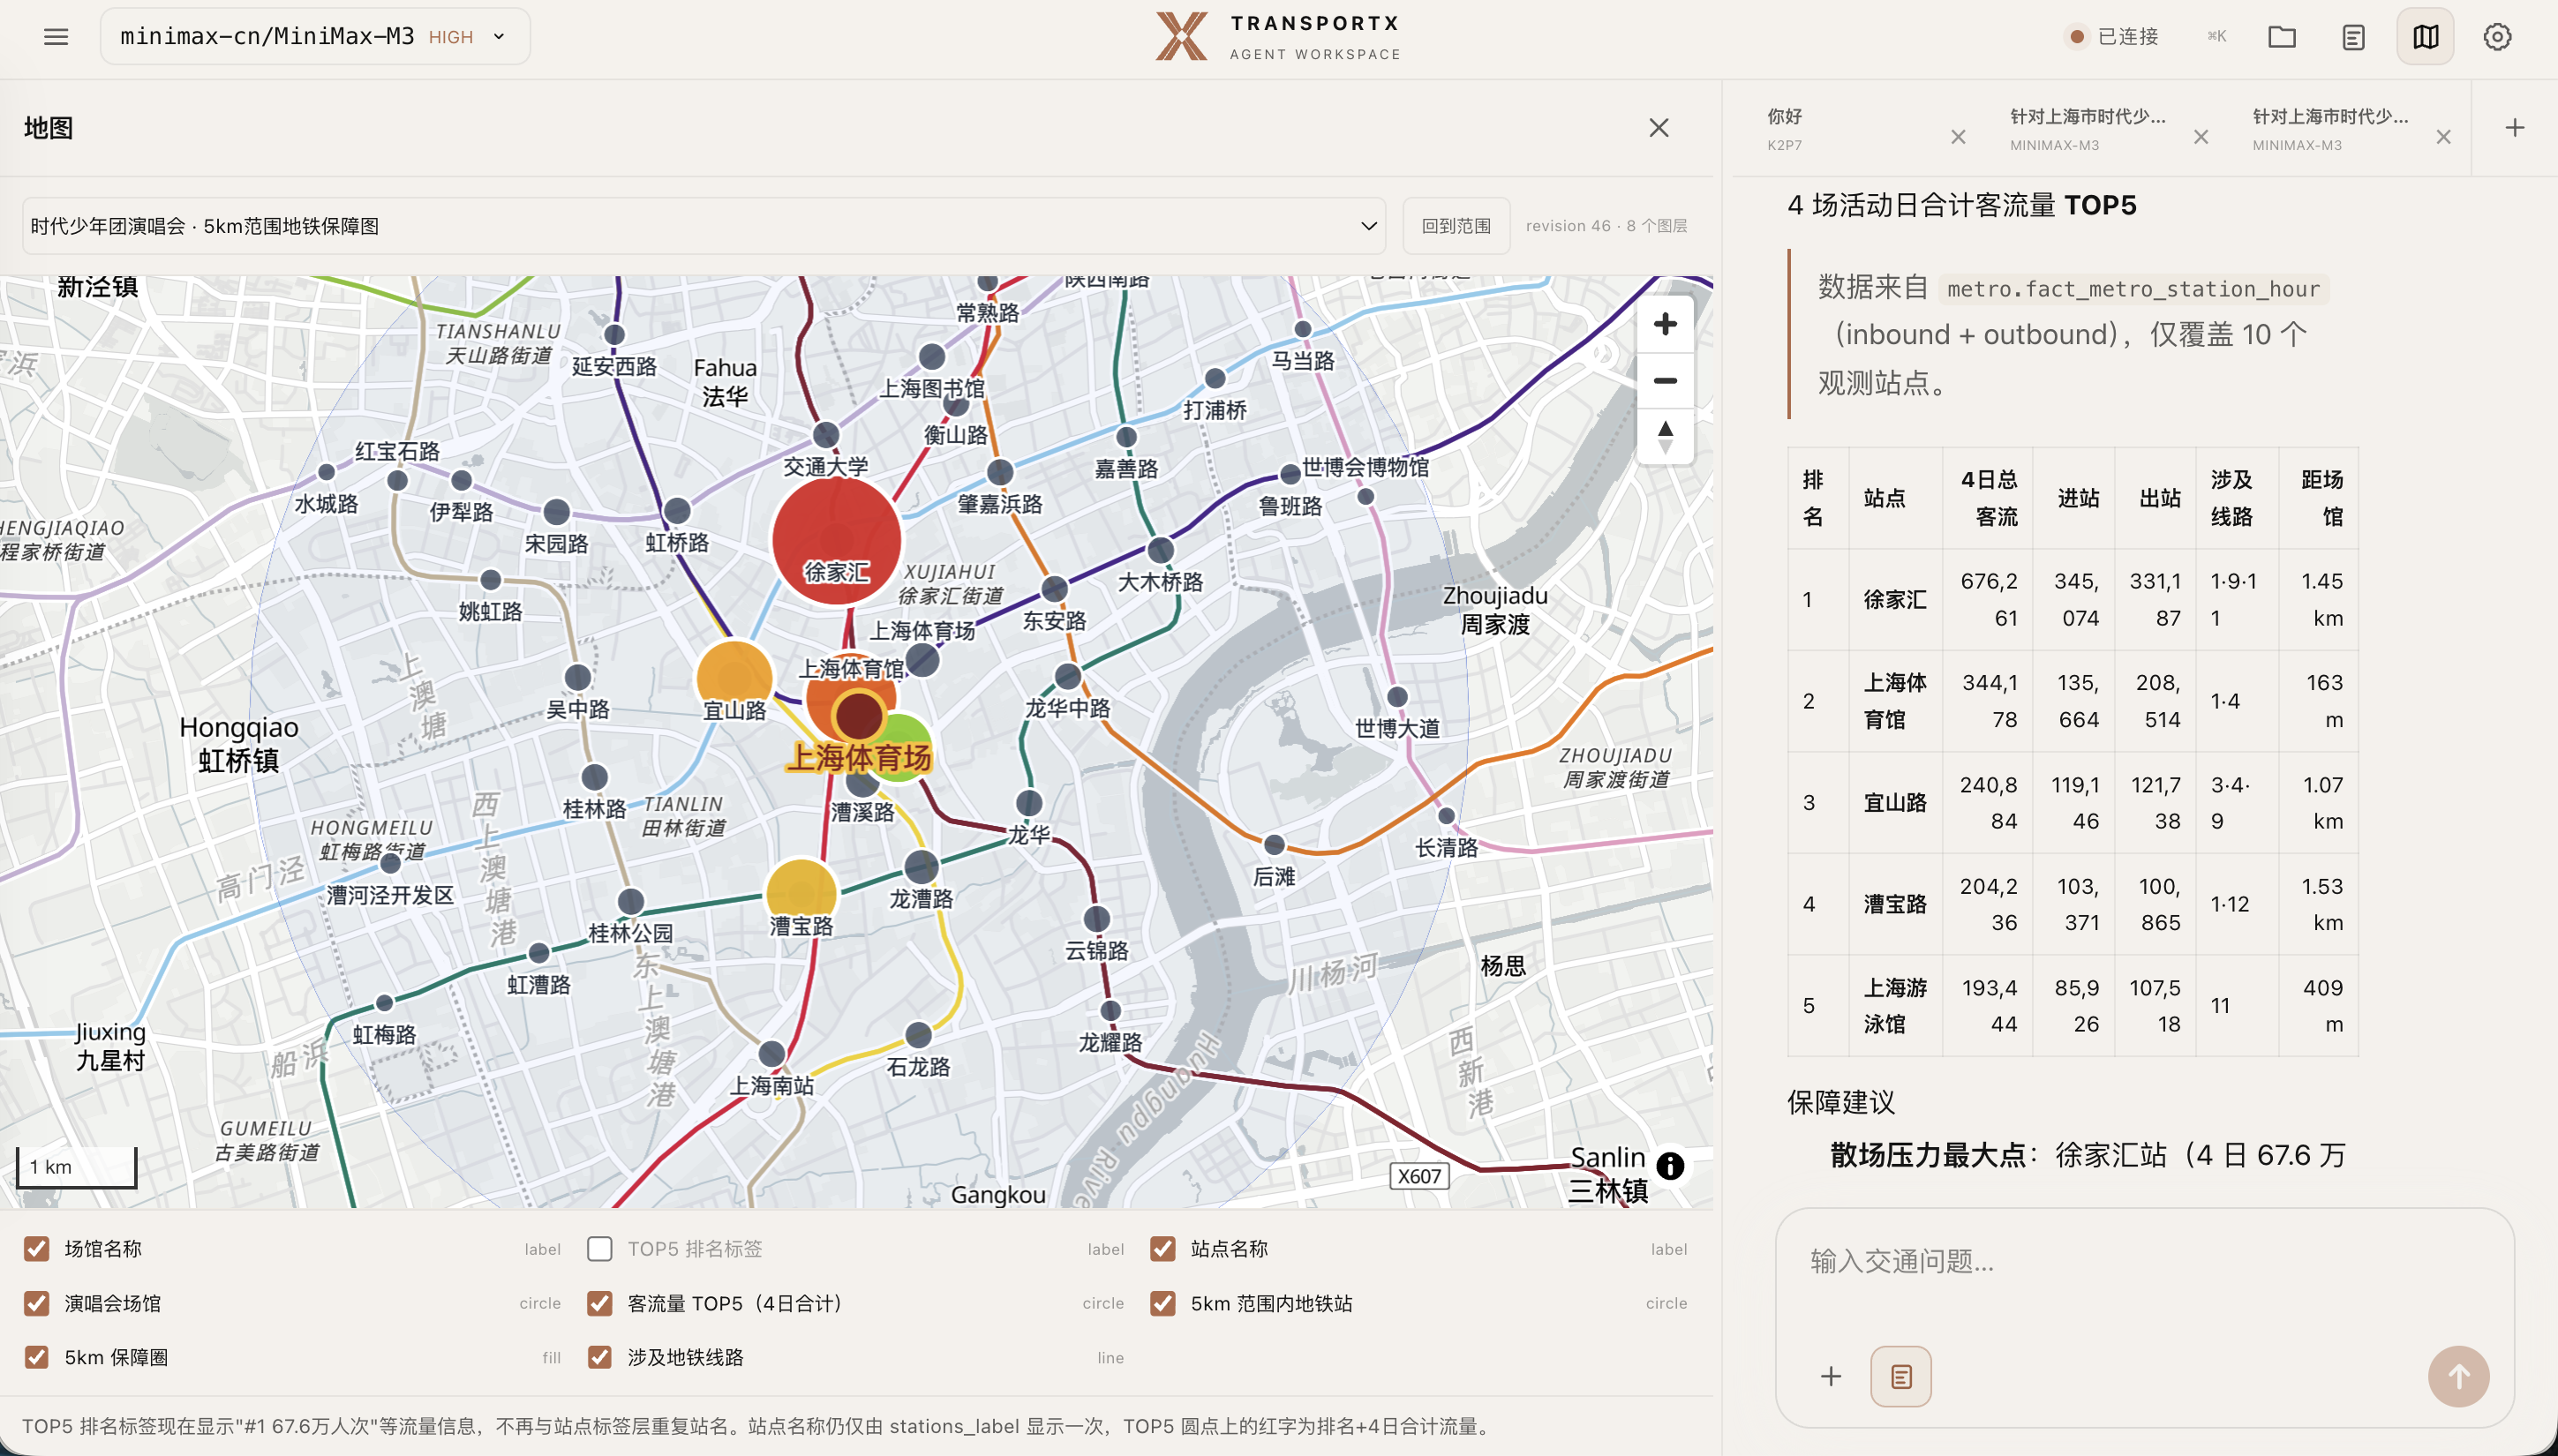
\includegraphics[width=0.92\linewidth]{02-metro-保障图.png}
  \caption{场馆 5 km 范围轨交保障图与四场活动日客流 TOP5}
  \label{fig:metro}
\end{figure}

\begin{figure}[ht]
  \centering
  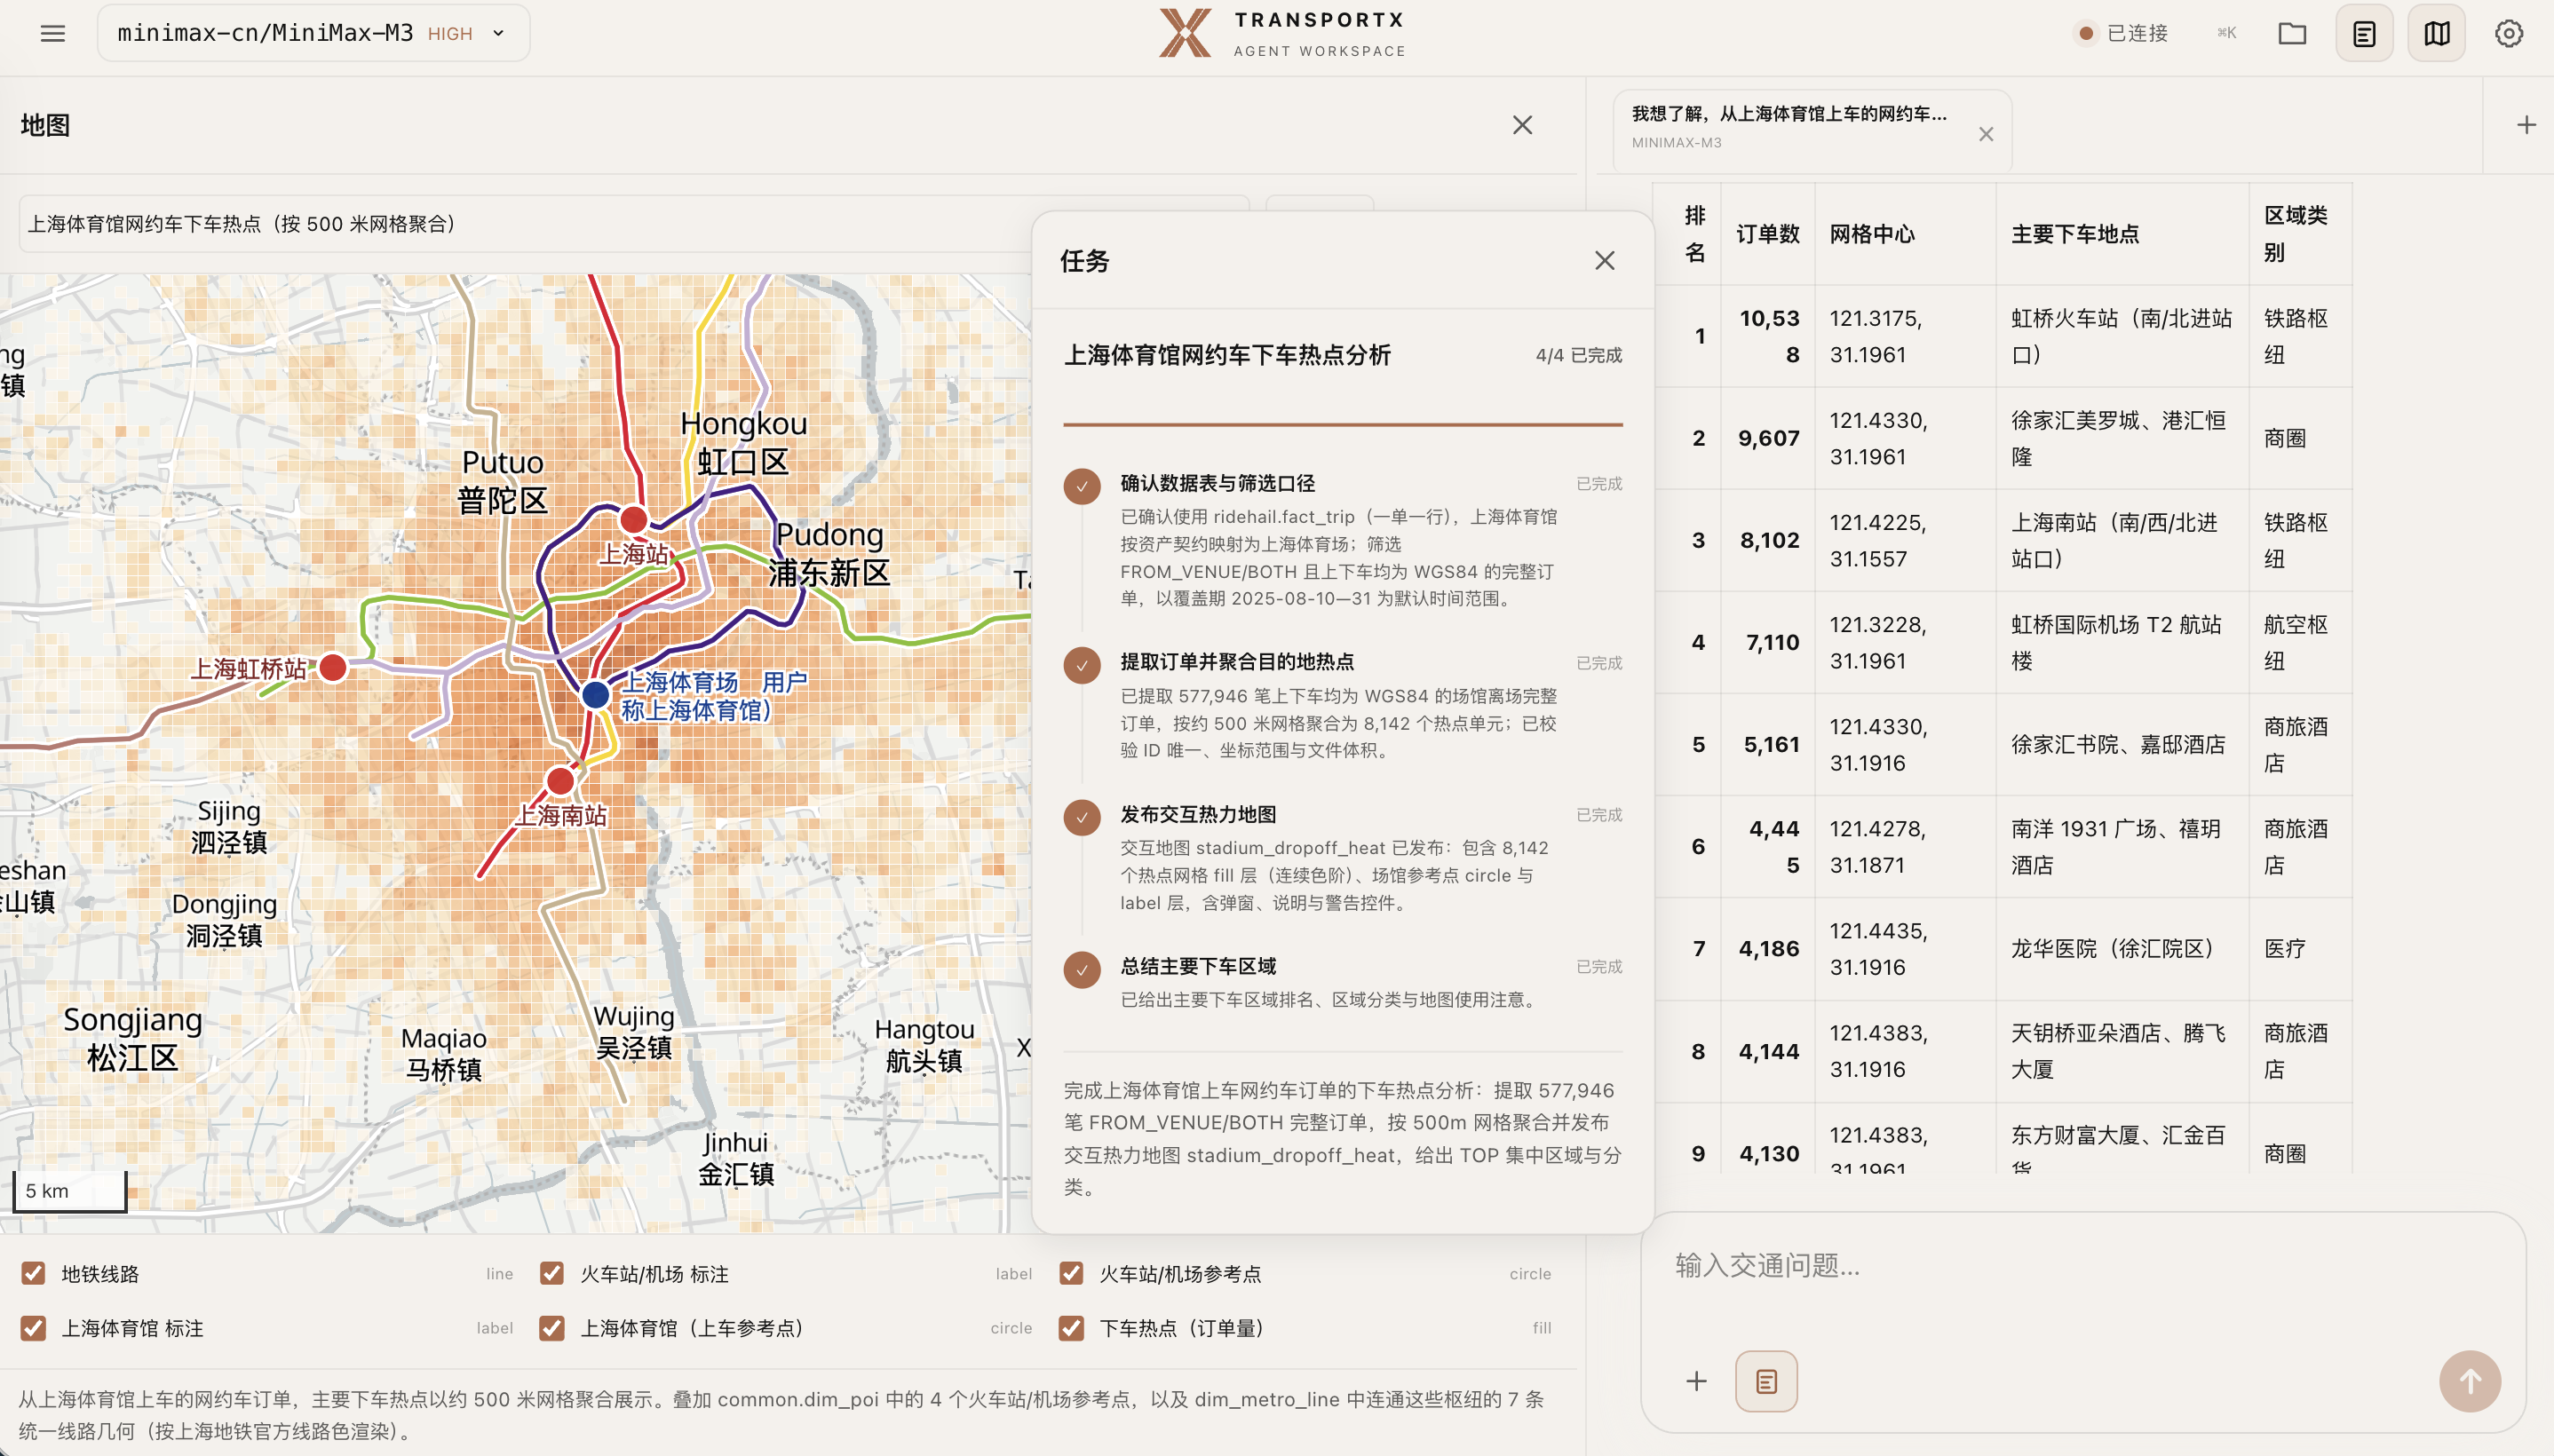
\includegraphics[width=0.92\linewidth]{03-ridehail-dropoff-heatmap.png}
  \caption{散场网约车下车热点、重要场站与轨交线路叠加分析}
  \label{fig:ridehail}
\end{figure}

\begin{figure}[ht]
  \centering
  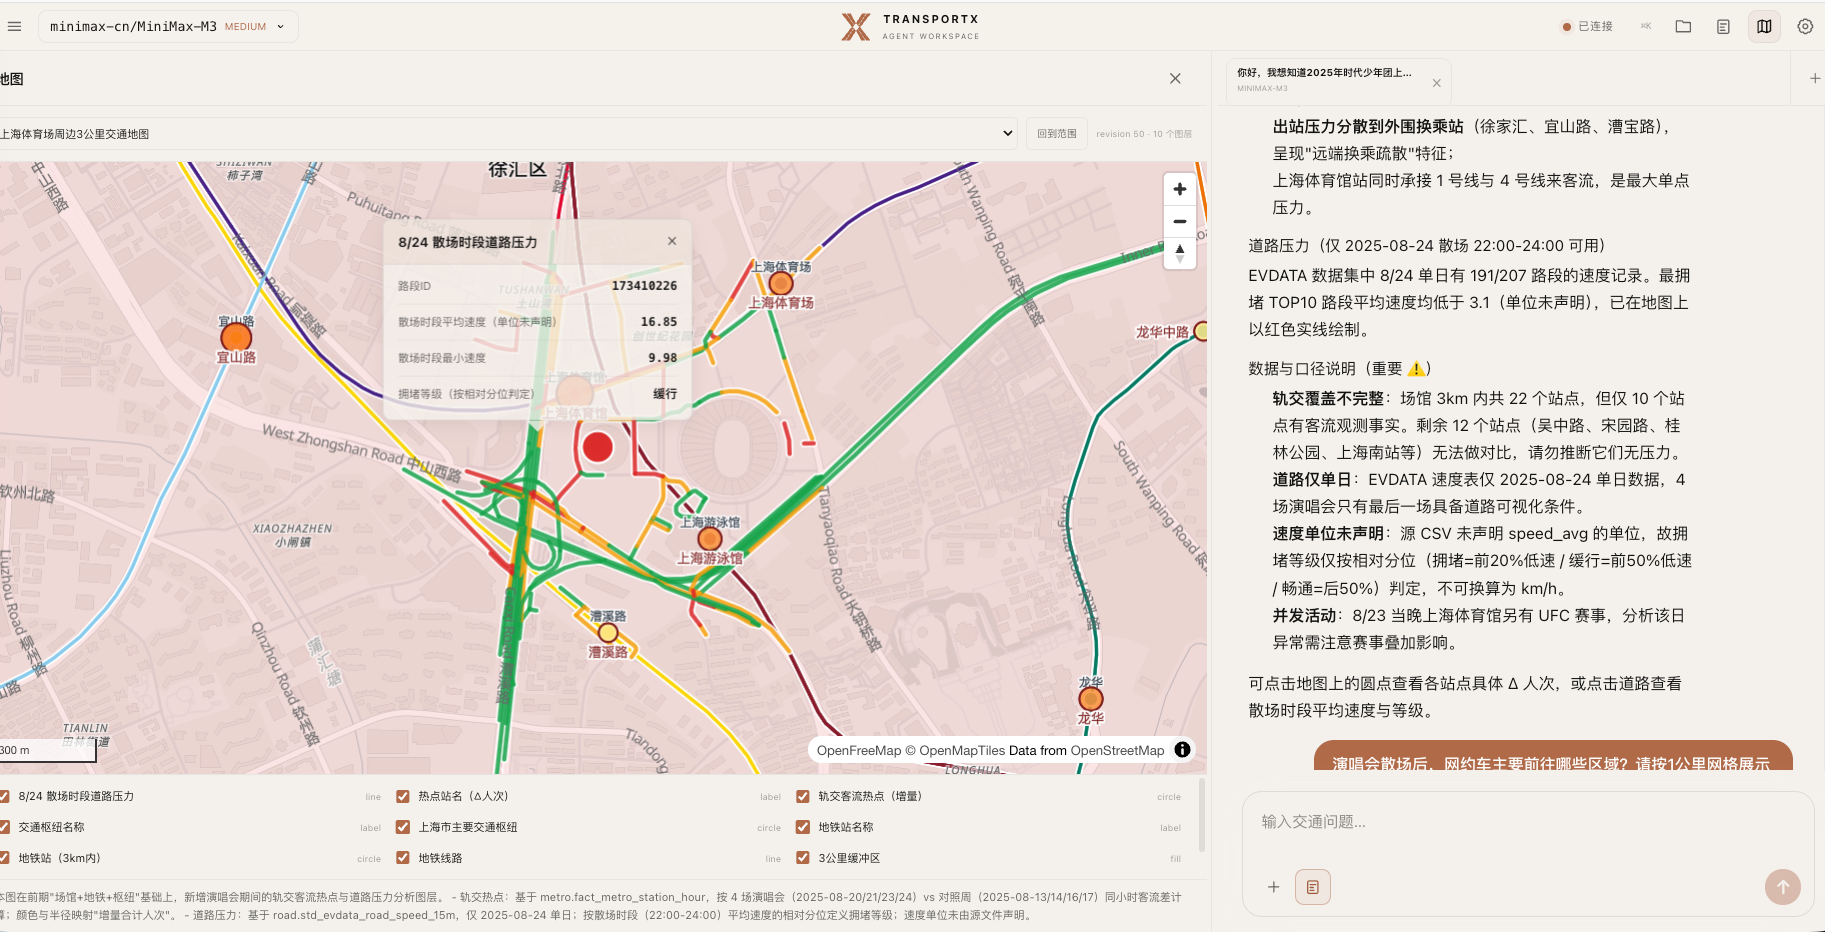
\includegraphics[width=0.92\linewidth]{06-evdata-road-pressure.png}
  \caption{散场时段道路压力专题图与站点点击详情（基于 EVDATA 数据）}
  \label{fig:evdata}
\end{figure}

\begin{figure}[ht]
  \centering
  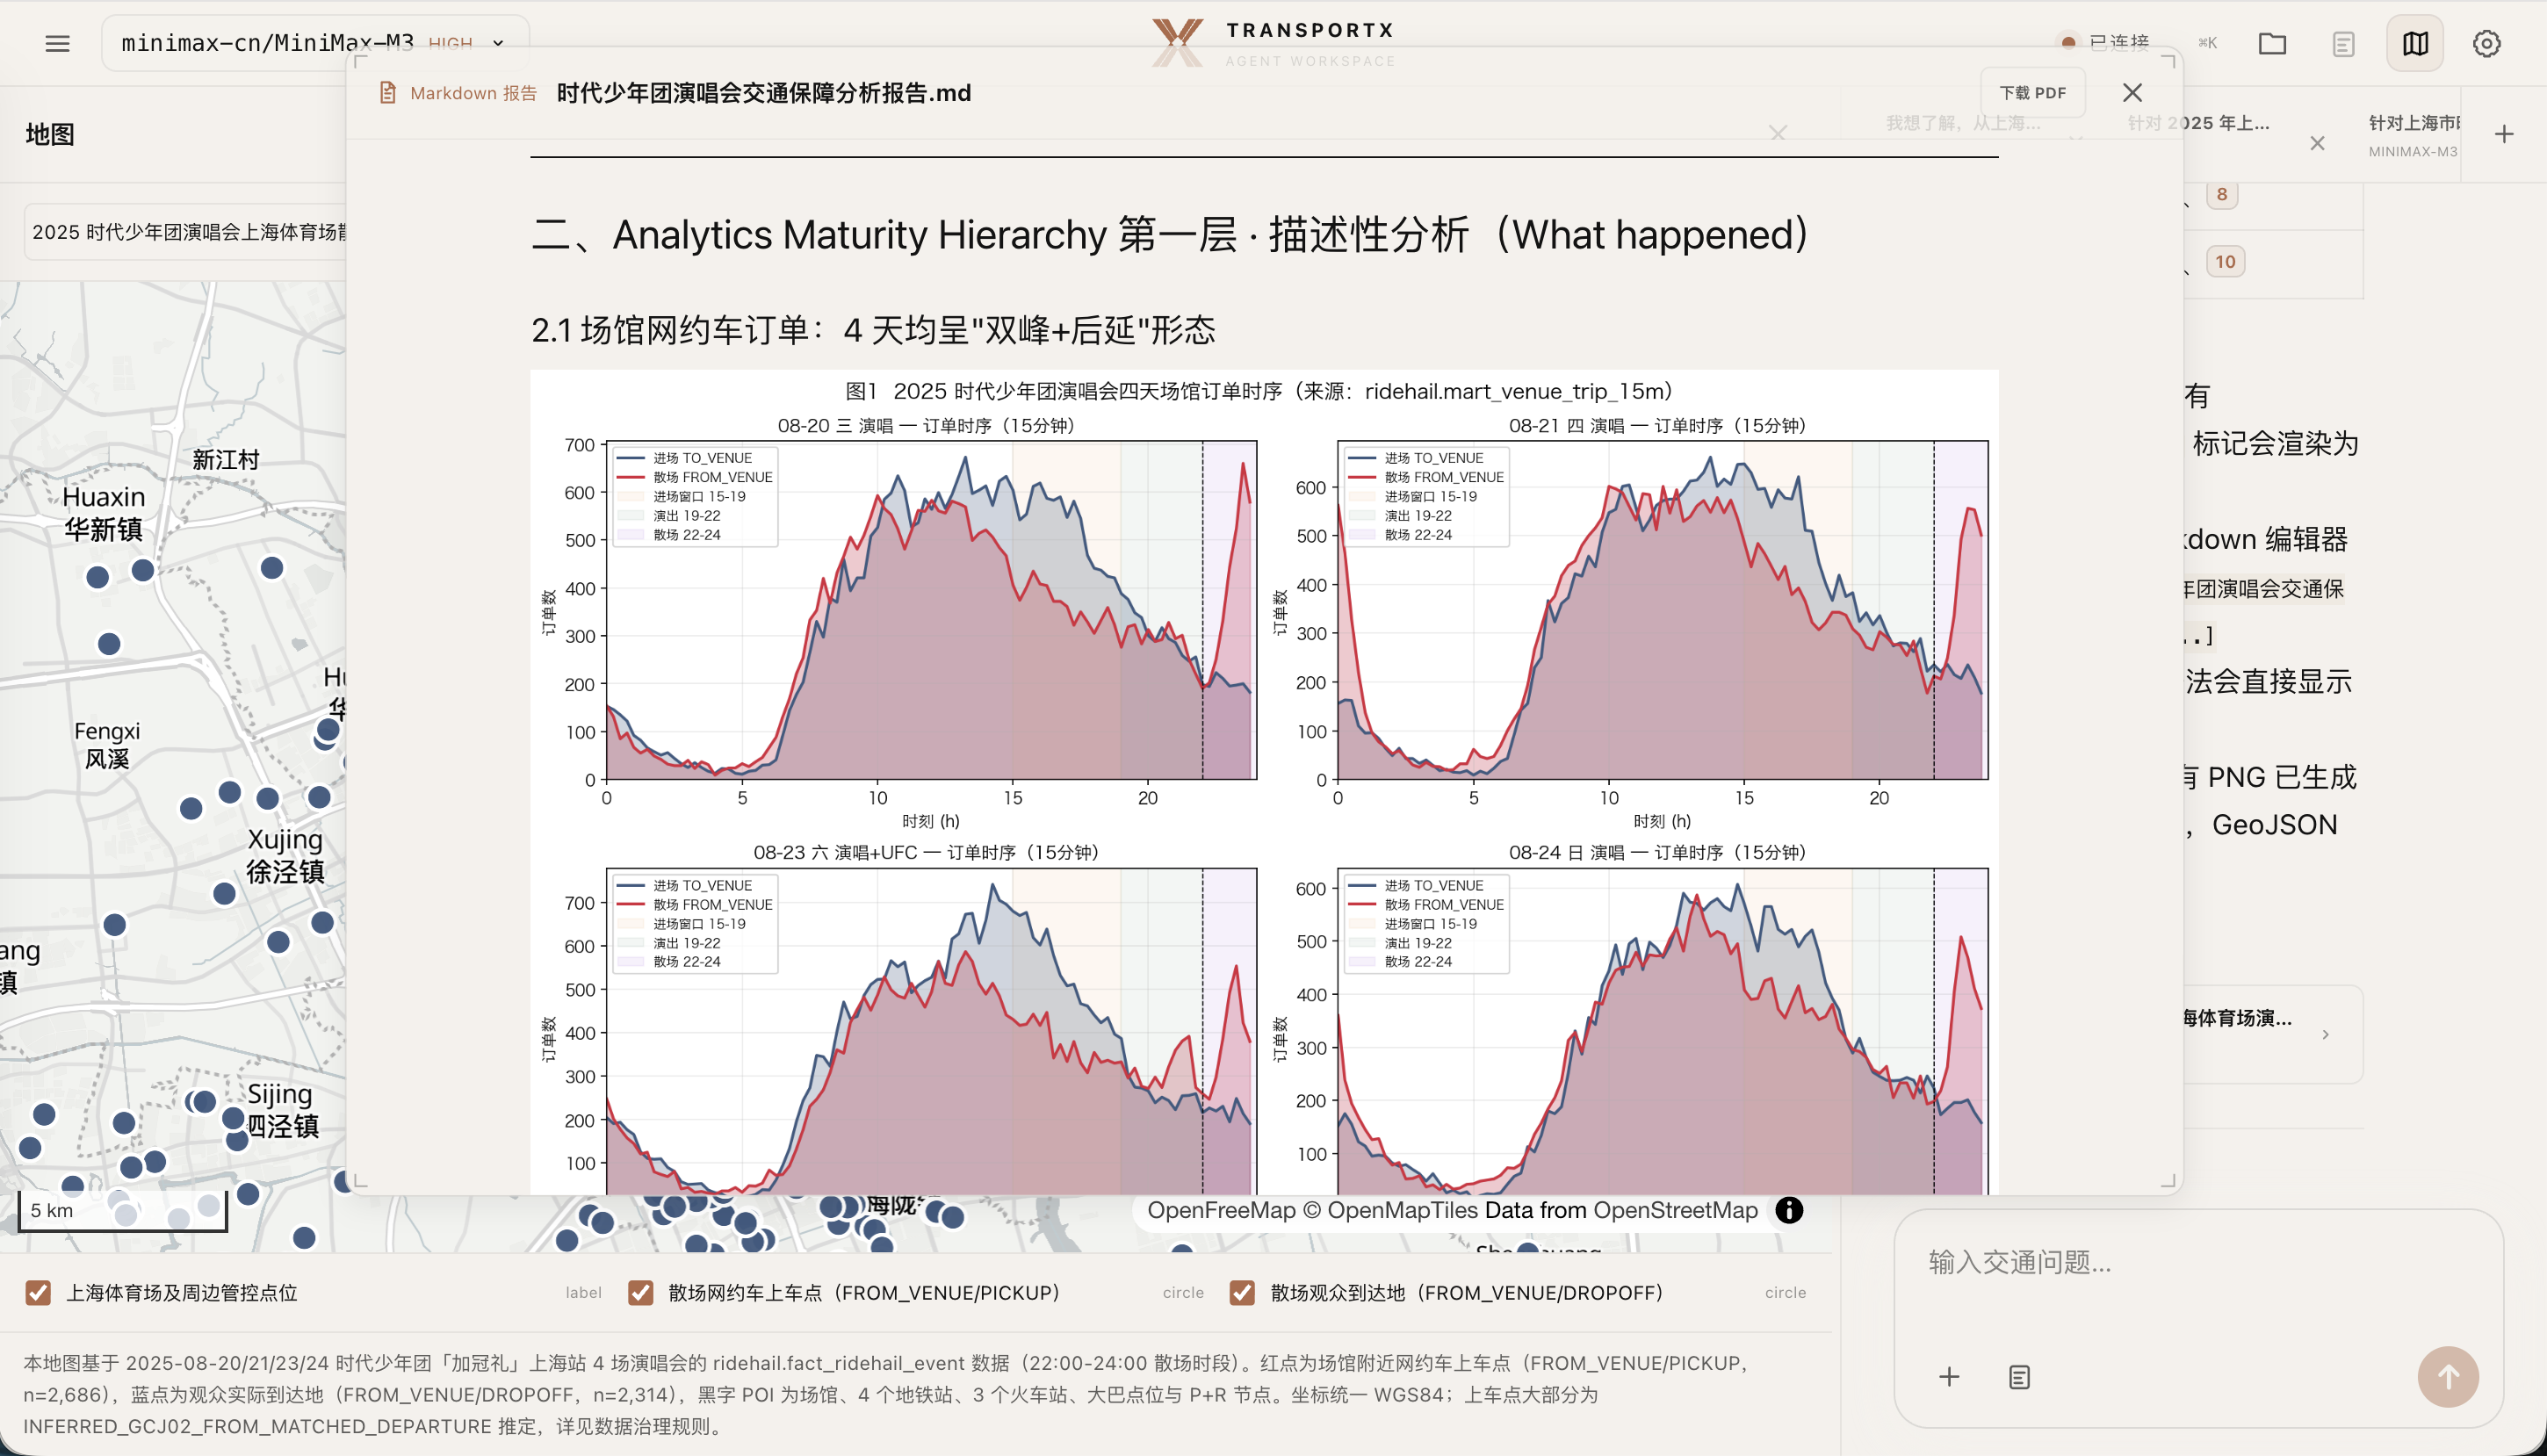
\includegraphics[width=0.92\linewidth]{04-report-preview.png}
  \caption{同一会话内的报告预览与导出}
  \label{fig:report}
\end{figure}

\begin{figure}[ht]
  \centering
  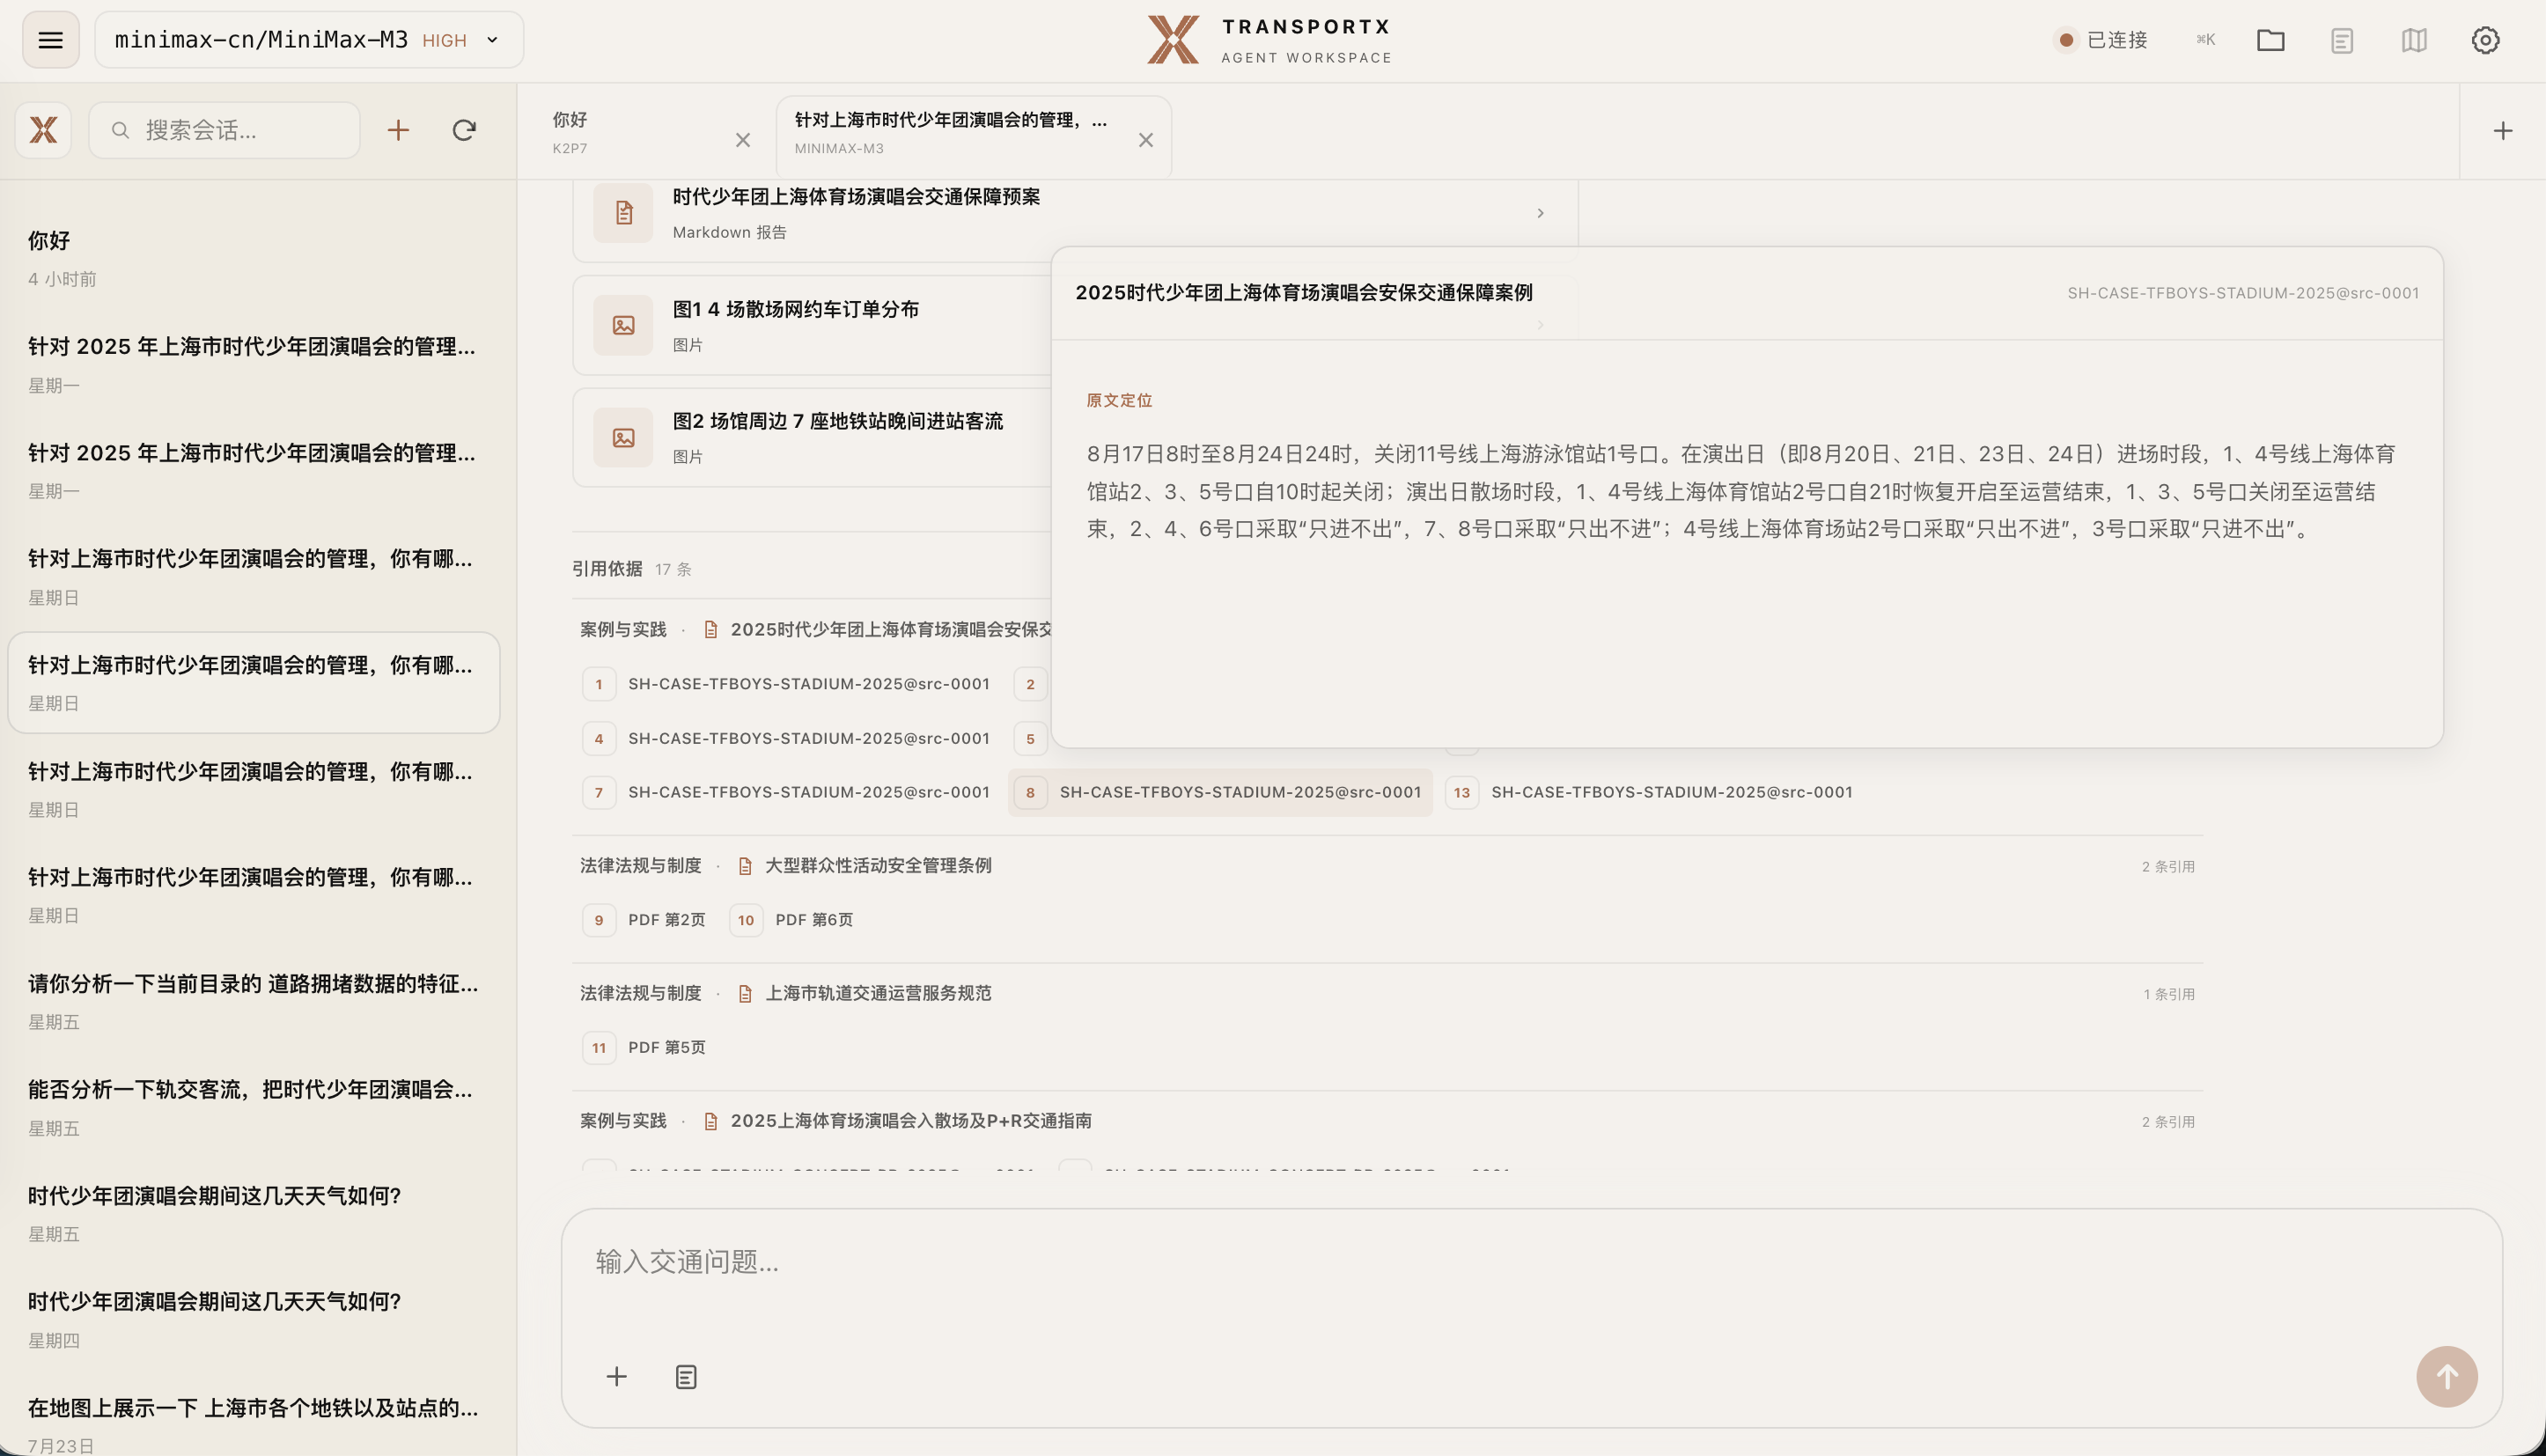
\includegraphics[width=0.92\linewidth]{05-citation-detail.png}
  \caption{引用清单与法规、预案原文定位}
  \label{fig:citation}
\end{figure}

围绕同一份任务，业务人员可以在对话中查看结论、在地图上核查分布、在任务看板中追溯步骤、在文件工作区打开报告与引用，所有数据来源、操作命令和图表脚本一并保存。

\subsection{已知缺陷与边界说明}

\begin{itemize}
  \item \term{数据时间跨度：}各事实域约 21—22 天，适用于活动期短周期对比。
  \item \term{空间覆盖：}轨交客流覆盖 10 个物理站；EVDATA 已入库 2025-08-24 单日样本；天气网格坐标系待确认。
  \item \term{部署范围：}当前版本适合本机或受控演示，多用户和局域网部署需要增加认证、授权、审计与配额。
\end{itemize}

% =============================================================================
%  八、成果交付清单
% =============================================================================
\section{成果交付清单}

\subsection{文档类交付物}

\begin{itemize}
  \item \term{项目建设说明报告：}完整说明项目建设内容、技术架构、数据治理、核心功能、可拓展性、安全合规、结果展示与已知缺陷。
  \item \term{系统架构说明：}记录系统边界、依赖方向和各模块职责。
  \item \term{数据资产说明与审查记录：}说明数据覆盖、字段结构、指标口径、空间信息和治理结果。
  \item \term{版本变更记录：}记录版本演进与验证结果。
\end{itemize}

\subsection{系统类交付物}

\begin{itemize}
  \item 交通态势智能工作台源码与构建脚本。
  \item Task Mode、Geo Visualization、Citation、Web Bridge 等扩展组件。
  \item 数据资产、地图绘制、知识检索等 Skill。
  \item 受控数据安装包（6 个 SQLite 分域库及治理脚本）。
\end{itemize}

\subsection{其他配套交付物}

仓库提供工作台首页、设置、命令面板、移动端和交通地图分析截图，可直接用于汇报；演示视频可按"新建交通任务—开启任务模式—完成问数—生成地图—导出报告"的路径录制。

\end{document}